\section{Using external devices \label{sec:external}}

Our third and last approach was to use an external device to compute the context switching time.
In this way, all the heavy computational processes are done outside of the benchmarked board.
This approach is later mentionned as the devices approach.

\subsection{Choice of the external device}

Our first idea was to implement it with Python3.7 on a desktop computer.
Using the Universal Asynchronous Receiver-Transmitter (UART) protocol over USB, the board sends a single byte containing the thread ID that is read by a Python script on the computer.

The motivations for using this alternative are:
\begin{itemize}
  \item Sending one byte of data over USB with UART have a smaller impact than computing the context switching time locally on the board;
  \item Time consuming computational tasks of the framework are done on the computer and not on the board;
  \item Using Python3.7, we can achieve a time precision at the nanosecond.
\end{itemize}

However, after discussing with the embedded community, we abandonned this idea for the following reasons:
\begin{itemize}
  \item There is buffering happening on the USB-serial chip on the board, on the PC's USB hardware, in the PC USB-serial driver 
    and also in the desktop operating systems;
  \item Those buffering will add delay in our measurements;
  \item Context switches will occur on the desktop computer that will invalidate any timing value.
\end{itemize}


Instead, we decided to use a device called the Pocket Science Lab (PSLab) to perform our experiments.

\begin{figure}[!ht]
  \centering
  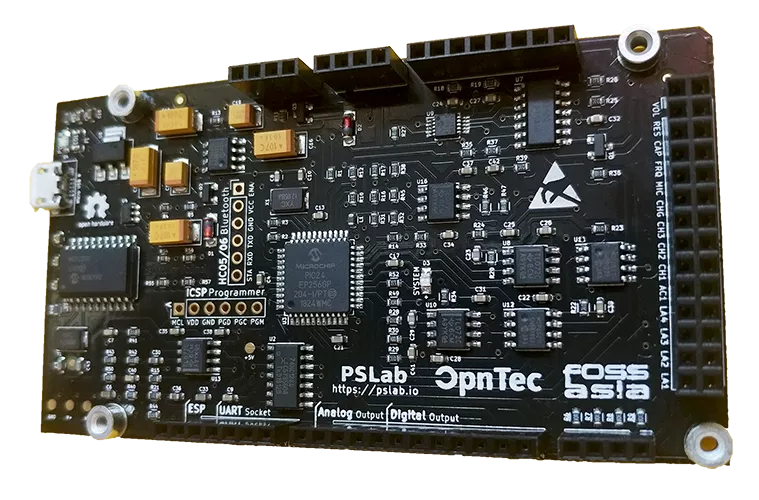
\includegraphics[scale=0.25]{assets/pslab.png}
  \caption{\label{fig:pslab}Pocket Science Lab device from PSLab.io}
\end{figure}

The Pocket Science Lab device from PSLab.io\footnote{\url{https://pslab.io}} comes 
  with a built-in 4-Channel up to 2MSPS oscilloscope, multimeter, 4-Channel, 4 MHz logic analyser, and other digital instruments.
Using the Python library \texttt{pslab-python}\footnote{\url{https://github.com/fossasia/pslab-python}}, we can communicate with the board and experiment with it.
With a device like the PSLab, we can leave the benchmarked board that contains our simple application untouched in terms of heavy computations.

\subsection{Role of the different devices}

With the benchmarked board, the PSLab and the computer, we have three devices that we use to compute the context switching time.
The figure \ref{fig:external-benchmarking-framework-schema} shows the connections between the different devices.
To make some clarity, we have defined a specific role to each device.

\subsubsection{The benchmarked board}
The benchmarked board runs the RTOS of our choice with the benchmarking framework and the simple application.
It communicates with the computer through UART and with the PSLab using a single GPIO.
The GPIO channel is used for timing computation while the UART channel is used to flash and read any serial output from the board by the computer.
Its role is to simply run the application and change the state of the GPIO depending on the tasks status.

\subsubsection{The computer}
The computer is the brain of the benchmarking framework.
It is responsible of communicating with both the benchmarked board and the PSLab through the UART protocol.
It coordinates the benchmarked board and the PSLab in order to retrieve the context switching time.
The computer is also the place where all the data are gathered.

\subsubsection{The PSLab}
Connected with a single GPIO to the benchmarked board, the PSLab watches for any context switch.
It measures the context switching time using its logical analyzer.
The board receives its instructions and sends the measures through UART with the computer.

\begin{figure}[!ht]
  \centering
  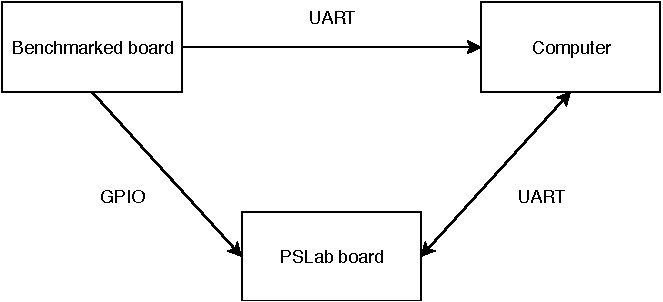
\includegraphics[scale=1]{assets/external-benchmarking-framework-schema.pdf}
  \caption{\label{fig:external-benchmarking-framework-schema}interaction schema of the devices used in the framework}
\end{figure}

\subsection{Usage of the Pocket Science Lab}

The PSLab monitors a single GPIO and measures the context switching time from it.
The figure \ref{fig:external-framework-context-switching-time-measurement} shows the steps in the measurement with the PSLab.
Each task will set the GPIO up at the start of its execution and then reset the GPIO once it ended.
In our example, the task 1 set up the GPIO at the step A and the GPIO is in high position at step A'.
Once the task 1 is finished, it reset the GPIO at the step B that will be in low position at step B'.
The same process occurs for the task 2.
The task 2 set up the GPIO at step C.
The GPIO is in high position at step C'.
Finally, the task 2 reset the GPIO at the end of its execution at step D and the GPIO will be in position low at step D'.
From our measurements made with the reference value, we know that the rising and falling times of the GPIO is around 10 nanoseconds so it can be omitted.

\begin{figure}[!ht]
  \centering
  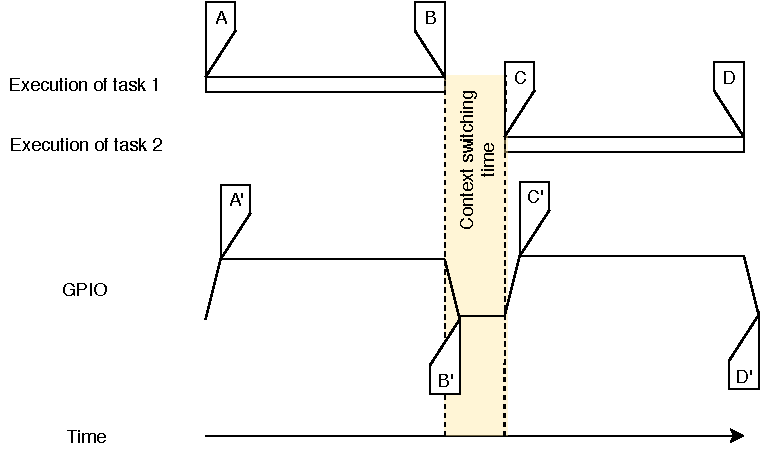
\includegraphics[scale=1]{assets/external-framework-context-switching-time-measurement.pdf}
  \caption{\label{fig:external-framework-context-switching-time-measurement}measurement of the context switching time with a single GPIO}
\end{figure}

\subsection{Using the framework with our simple application}

To understand the framework implementation, it is important to understand what happens when our simple application boots, 
  both from the point of view of the benchmarked board and from the point of view of the PSLab and the computer.

\subsubsection{Point of view of the benchmarked board}
When the application boots, it will initialize the framework.
An initializiation is required to use the GPIO.
Once the initializiation is done, the first task starts.
It will call \texttt{bench\_on()} from the framework.
In the framework-space, \texttt{bench\_on()} will have for effect to set the GPIO up.
When the task is done, it will call \texttt{bench\_off()} that will reset the GPIO.
The second task goes in the foreground and will also call \texttt{bench\_on()} and, latter, \texttt{bench\_off()}.

\subsubsection{Point of view of the PSLab and the computer}
The PSLab will listen for an interval between a falling and a rising edge.
In the figure \ref{fig:external-framework-context-switching-time-measurement}, this interval happens between the step B' and C'.
For reminder, the rising time can be omitted.
Once the PSLab detects an interval, it computes its duration.
This interval time is the context switching time.
This measure is sent to the computer that will store it.

\subsection{Framework implementation}

The interaction between the benchmarked board and the PSLab is done through a GPIO that is controlled by the benchmarked board.
The code in the benchmarked board is quite straightforward.
First, our simple application needs to initialize the framework and start its tasks.
Then, we need to add \texttt{bench\_on()} and \texttt{bench\_off()} respectively at the start and at the end of the two tasks.
The code of the updated application is shown in the listing \ref{lst:external-app-code}.

\begin{lstlisting}[style=CStyle, float, caption={source code of the simple application in Contiki}, label={lst:external-app-code}]
#include "contiki.h"
#include "sys/clock.h"
#include "bench-context-switching.h"

#include <stdio.h>

PROCESS(init_task, "Init task");
PROCESS(task_1, "First task");
PROCESS(task_2, "Second task");
AUTOSTART_PROCESSES(&init_task);

PROCESS_THREAD(init_task, ev, data)
{
    PROCESS_BEGIN();

    bench_init();

    process_start(&task_1, NULL);
    process_start(&task_2, NULL);

    PROCESS_END();
}

PROCESS_THREAD(task_1, ev, data)
{
    PROCESS_BEGIN();

    while (1)
    {
        bench_on();
        clock_delay_usec(1000);
        bench_off();
        PROCESS_PAUSE();
    }

    PROCESS_END();
}

// ...
// task_2 is identical to task_1
\end{lstlisting}

During the initializiation, the framework will setup the GPIO as an output port. 
The listing \ref{lst:external-init-code} shows this process.
The \texttt{bench\_on()} and \texttt{bench\_off()} will just set or reset the GPIO like shown in the listing \ref{lst:external-on-off-code}.

\begin{lstlisting}[style=CStyle, caption={initializiation of the framework in Contiki}, label={lst:external-init-code}]
void bench_init()
{
    GPIO_SOFTWARE_CONTROL(GPIO_PORT_TO_BASE(GPIO_C_NUM), GPIO_PIN_MASK(2));
    GPIO_SET_OUTPUT(GPIO_PORT_TO_BASE(GPIO_C_NUM), GPIO_PIN_MASK(2));
}
\end{lstlisting}

\begin{lstlisting}[style=CStyle, caption={\texttt{bench\_on()} and \texttt{bench\_off()} implementation in Contiki}, label={lst:external-on-off-code}]
void bench_on(uint32_t pid)
{
    GPIO_SET_PIN(GPIO_PORT_TO_BASE(GPIO_C_NUM), GPIO_PIN_MASK(2));
}

void bench_off()
{
    GPIO_CLR_PIN(GPIO_PORT_TO_BASE(GPIO_C_NUM), GPIO_PIN_MASK(2));
}
\end{lstlisting}

Finally, from the computer, we need to retrieve and store the interval measurements from the PSLab.
To do so, we use a Python script shown in listing \ref{lst:python-pslab} that connects to the PSLab and retrieves the context switching time between a falling and a rising edge.

The complete source code can be found on the Github repository\footnote{\url{https://github.com/bench-os/bench-os}}.

\begin{lstlisting}[style=CStyle, language=python, caption={Python script to communicate with the PSLab and retrieve the interval measurements}, label={lst:python-pslab}]
from PSL import sciencelab
I = sciencelab.connect()

VALUES = []

while True:
    CS_TIME = I.MeasureInterval('ID1', 'ID1', 'falling', 'rising')
    VALUES.append(CS_TIME)
\end{lstlisting}